\begin{figure}[H]
  \begin{center}
    \centering
    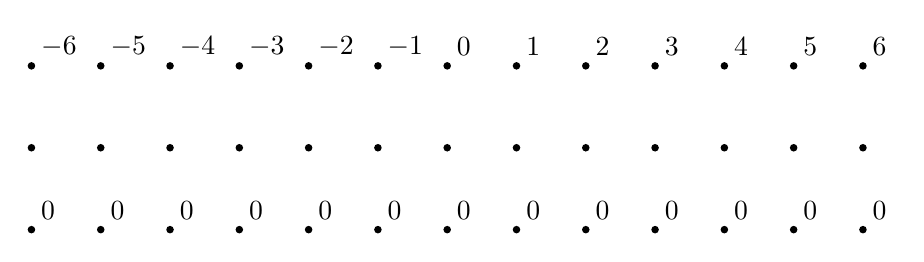
\begin{tikzpicture}[scale=0.8]
      \foreach \y in {1, 0, -1} {
          \foreach \x in {-6, ..., 6} {
              \fill[color=black] (\x*1.1+3,\y*1.3) circle (0.06);

              \ifnum\y=1
                \node[right] at (\x*1.1+3,\y*1.3+0.3) {$\x$};
              \fi
              \ifnum\y=-1
                \node[right] at (\x*1.1+3,\y*1.3+0.3) {$0$};
              \fi
            }
        }
    \end{tikzpicture}
    \captionsetup{justification=centering}
    \caption{
      \pt{Função $1$-limitada sem extensão $\alpha$-limitada, para qualquer $\alpha > 0$, para um conjunto com infinitos pontos adicionais.}
      \en{$1$-bounded function without an $\alpha$-bounded extension, for any $\alpha > 0$, for a set with infinitely many additional points.}
    }
  \end{center}
\end{figure}
